\documentclass[tikz,border=2mm]{standalone}
\usetikzlibrary{perspective}

\tikzset
{
  cylinder back/.style={left color=blue,right color=white,fill opacity=0.3},
  cylinder front/.style={left color=white,right color=blue,fill opacity=0.6},
  sphere/.style={shading=ball,ball color=red,fill opacity=0.7}
}

\begin{document}
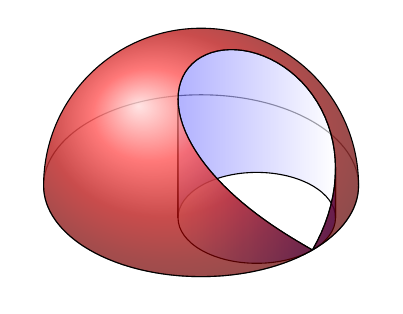
\begin{tikzpicture}[isometric view,rotate around z=180,line join=round]
  % tangent points 
  \coordinate (R1) at ({cos(135)},{1+sin(135)},0);                    % right, bottom
  \coordinate (L2) at ({cos(-45)},{1+sin(-45)},{sqrt(2-2*sin(-45))}); % left,  top
  % base circle
  \draw[gray] (0,0) circle (2);
  % cylinder
  \draw[cylinder back]  (R1) arc (135:315:1) -- (L2) --
     plot[domain=315:135,samples=37]({cos(\x)},{1+sin(\x)},{sqrt(2-2*sin(\x))}) -- cycle; 
  \draw[cylinder front] (R1) arc (135:-45:1) -- (L2) --
     plot[domain=-45:135,samples=37]({cos(\x)},{1+sin(\x)},{sqrt(2-2*sin(\x))}) -- cycle; 
  % sphere  
  \draw[sphere] (0,2) arc (90:-45:2) arc (180:0:2cm) arc (135:90:2) 
     plot[domain=0:360,samples=73]({cos(\x)},{1+sin(\x)},{sqrt(2-2*sin(\x))});
\end{tikzpicture}
\end{document}